\caulc
%%%=============EX_1=============%%%
\begin{ex}%[1D6H4-3]%[TDMZZ10]%[Mui Doan]
	Tập nghiệm của bất phương trình $\log_2(3x-1)<3$ là
	\choice
	{\True $\left(\dfrac{1}{3};3\right)$}
	{$(0;2)$}
	{$(1;4)$}
	{$(2;6)$}
	\loigiai{
		Điều kiện $3x-1>0\Leftrightarrow x>\dfrac{1}{3}$.\\
		Ta có $\log_2(3x-1)<3\Leftrightarrow 3x-1<8\Leftrightarrow x<3$.\\
		So điều kiện ta có $x\in \left(\dfrac{1}{3};3\right)$.
	}
\end{ex}
%%%=============================%%%

%%%=============EX_2=============%%%
\begin{ex}%[1D7N2-1]%[TDMZZ10]%[Mui Doan]
	Đạo hàm của hàm số $y=2^x$ là
	\choice
	{\True $y'=2^x\ln 2$}
	{$y'=2^x$}
	{$y'=\dfrac{2^x}{\ln 2}$}
	{$y'=x2^{x-1}$}
	\loigiai{
		Ta có $y'=2^x\ln 2$.
	}
\end{ex}
%%%=============================%%%

%%%=============EX_3=============%%%
\begin{ex}%[1H8H7-4]%[TDMZZ10]%[Nguyễn Vương]
	Cho hình lăng trụ đứng $ABC. A'B'C'$ có đáy là tam giác đều và có mặt bên là hình vuông có diện tích bằng $16$. Thể tích của $ABC. A'B'C'$ bằng
	\choice
	{$4\sqrt{3}$}
	{$24$}
	{$8\sqrt{6}$}
	{\True $16\sqrt{3}$}
	\loigiai{
		Vì các mặt bên của lăng trụ đứng có đáy tam giác đều là các hình chữ nhật bằng nhau, mà có một mặt bên là hình vuông diện tích bằng $16$ nên tất cả các cạnh của lăng trụ đều bằng $4$.\\
		Diện tích đáy của lăng trụ là $S = \dfrac{4^2\sqrt{3}}{4} = 4\sqrt{3}$.\\
		Thể tích của lăng trụ là $V = S \cdot h = 4\sqrt{3} \cdot 4 = 16\sqrt{3}$.
	}
\end{ex}
%%%=============================%%%

%%%=============EX_4=============%%%
\begin{ex}%[1D2H2-2]%[TDMZZ10]%[Nguyễn Tấn Linh]
	Cho cấp số cộng $(u_n)$ có tổng hai số hạng đầu bằng $3$ và tổng ba số hạng đầu bằng $6$. Công sai của $(u_n)$ bằng
	\choice
	{$3$}
	{$2$}
	{\True $1$}
	{$4$}
	\loigiai{
		Gọi $u_1$ là số hạng đầu và $d$ là công sai của cấp số cộng $(u_n)$.\\
		Ta có hệ phương trình $\heva{&u_1+u_2=3\\&u_1+u_2+u_3=6} \Leftrightarrow \heva{&2u_1+d=3\\&3u_1+3d=6} \Leftrightarrow \heva{&u_1=1\\&d=1.}$\\
		Vậy công sai của cấp số cộng là $d=1$.
	}
\end{ex}
%%%=============================%%%

%%%=============EX_5=============%%%
\begin{ex}%[2D3N1-2]%[TDMZZ10]%[Nguyễn Tấn Linh]
	Cho mẫu số liệu ghép nhóm $M$ với bảng tần số ghép nhóm như sau:
	\begin{center}
		\begin{tabular}{|c|c|c|c|c|c|c|}
			\hline
			\textbf{Nhóm} & $[8;10)$ & $[10;12)$ & $[12;14)$ & $[14;16)$ & $[16;18)$ & $[18;19)$ \\
			\hline
			\textbf{Tần số} & $6$ & $6$ & $8$ & $4$ & $6$ & $7$ \\
			\hline
		\end{tabular}
	\end{center}
	Hãy xác định khoảng biến thiên của mẫu số liệu $M$?
	\choice
	{$12$}
	{\True $11$}
	{$19$}
	{$8$}
	\loigiai{
		Khoảng biến thiên của mẫu số liệu ghép nhóm là hiệu số giữa đầu mút phải của nhóm cuối cùng và đầu mút trái của nhóm đầu tiên.\\
		Ta có $R = 19 - 8 = 11$.
	}
\end{ex}
%%%=============================%%%

%%%=============EX_6=============%%%
\begin{ex}%[2D1N4-1]%[TDMZZ10]%[Bồ Văn Hậu]
	Số đường tiệm cận của đồ thị hàm số $y = \dfrac{2x-1}{3x+1}$ là
	\choice
	{\True $2$}
	{$1$}
	{$0$}
	{$3$}
	\loigiai{
		Ta có
		\begin{itemize}
			\item $\displaystyle \lim\limits_{x \to -\infty} \dfrac{2x-1}{3x+1}=\dfrac{2}{3}$ và $\displaystyle \lim\limits_{x \to +\infty} \dfrac{2x-1}{3x+1}=\dfrac{2}{3}$ hay đồ thị có $1$ đường tiệm cận ngang $y=\dfrac{2}{3}$.
			\item $\displaystyle \lim\limits_{x \to \left(-\dfrac{1}{3}\right)^+}\dfrac{2x-1}{3x+1}=-\infty$ và $\displaystyle \lim\limits_{x \to \left(-\dfrac{1}{3}\right)^-}\dfrac{2x-1}{3x+1}=+\infty$ hay đồ thị có $1$ đường tiệm cận đứng $x = -\dfrac{1}{3}$.
		\end{itemize}
		Vậy tổng số đường tiệm cận của đồ thị hàm số đã cho là $2$.
	}
\end{ex}
%%%=============================%%%

%%%=============EX_7=============%%%
\begin{ex}%[2D4N3-1]%[TDMZZ10]%[Bồ Văn Hậu]
	Cho hình phẳng $(H)$ giới hạn bởi các đường $y=f(x)$, trục $Ox$ và hai đường thẳng $x=a$, $x=b$ (với $a>b$). Diện tích hình phẳng $(H)$ được tính theo công thức
	\choice
	{$S=\displaystyle\int\limits_a^b f(x) \mathrm{\,d}x$}
	{$S=\displaystyle\int\limits_a^b \left|f(x)\right| \mathrm{\,d}x$}
	{\True $S=\displaystyle\int\limits_b^a \left|f(x)\right| \mathrm{\,d}x$}
	{$S=\pi \displaystyle\int\limits_0^1 \left[f(x)\right]^2 \mathrm{\,d}x$}
	\loigiai{
		Hình phẳng $(H)$ giới hạn bởi các đường $y=f(x)$, trục $Ox$ và hai đường thẳng $x=a$, $x=b$ (với $a>b$) có diện tích là $\displaystyle\int\limits_b^a \left|f(x)\right| \mathrm{\,d}x$.
	}
\end{ex}
%%%=============================%%%

%%%=============EX_8=============%%%
\begin{ex}%[2D1N5-1]%[TDMZZ10]%[Lê Phúc]
	\immini[thm]{Cho đồ thị hàm số $y=f(x)$ như hình vẽ bên dưới. Hỏi hàm số $f(x)$ có thể là hàm số nào dưới đây?
		\choice
		{$f(x)=ax^4+bx^2+c$}
		{$f(x)=ax^2+bx+c$}
		{\True $f(x)=ax^3+bx^2+cx+d$}
		{$f(x)=\dfrac{ax+b}{cx+d}$}}
	{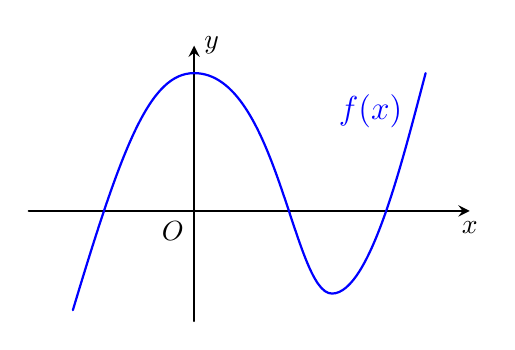
\begin{tikzpicture}[line join=round, line cap=round,>=stealth,thick,scale=.7]
			\draw[->] (-3,0) -- (5,0) node[below] {$x$};
			\draw[->] (0,-2) -- (0,3) node[right] {$y$};
			\node[below left] at (0,0) {$O$};
			\fill (0,0) circle (1pt);
			\draw[blue] 
			(-2.2, -1.8) 
			.. controls (-1.3, 1.2) and (-0.8, 2.5) .. (0, 2.5)
			.. controls (1.5, 2.5) and (1.8, -1.5) .. (2.5, -1.5)
			.. controls (3.2, -1.5) and (3.8, 1) .. (4.2, 2.5);
			\node[blue, font=\large] at (3.2, 1.8) {$f(x)$};
	\end{tikzpicture}}
	\loigiai{
		Dựa vào đồ thị hàm số ta có hàm số có $2$ cực trị và liên tục trên $\mathbb{R}$.\\
		Suy ra hàm số có thể là $f(x)=ax^3+bx^2+cx+d$.
	}
\end{ex}
%%%=============================%%%

%%%=============EX_9=============%%%
\begin{ex}%[2D4N1-3]%[TDMZZ10]%[Trần Văn Thiện]
	Họ nguyên hàm của hàm số $f(x)=\cos x$ là
	\choice
	{$F(x)=-\sin x+C$}
	{$F(x)=-\cos x+C$}
	{$F(x)=\cos x+C$}
	{\True $F(x)=\sin x+C$}
	\loigiai{
		Ta có $\displaystyle\int f(x)\mathrm{\,d}x=\displaystyle\int \cos x\mathrm{\,d}x=\sin x+C$, ($C$ là hằng số).
	}
\end{ex}
%%%=============================%%%

%%%=============EX_10=============%%%
\begin{ex}%[2H2N2-2]%[TDMZZ10]%[Đình Nguyên]
	Trong không gian $Oxyz$, khoảng cách từ điểm $A(2;2;-1)$ đến gốc tọa độ $O$ bằng
	\choice
	{$9$}
	{\True $3$}
	{$1$}
	{$5$}
	\loigiai{
		Gốc tọa độ có tọa độ là $O(0;0;0)$.\\
		Khoảng cách từ điểm $A(2;2;-1)$ đến gốc tọa độ $O$ là
		$OA = \sqrt{2^2 + 2^2 + (-1)^2} = \sqrt{9} = 3$.
	}
\end{ex}
%%%=============================%%%

%%%=============EX_11=============%%%
\begin{ex}%[2H5H3-2]%[TDMZZ10]%[Huỳnh Quốc Đạt]
	Trong không gian $Oxyz$, cho một mặt cầu $(S)$ có phương trình là $x^2 + y^2 + z^2 - 4x - 6y - 3 = 0$. Diện tích mặt cầu $(S)$ bằng
	\choice
	{$64\pi$}
	{\True $16\pi$}
	{$4\pi$}
	{$48\pi$}
	\loigiai{
		Ta có phương trình mặt cầu viết lại dưới dạng
		\[(x-2)^2 + (y-3)^2 + z^2 = 16.\]
		Suy ra bán kính mặt cầu $R = 4$.\\
		Diện tích mặt cầu $(S)$ là $S = 4\pi R^2 = 4\pi \cdot 16 = 64\pi$.
	}
\end{ex}
%%%=============================%%%

%%%=============EX_12=============%%%
\begin{ex}%[2H2H1-2]%[TDMZZ10]%[Nguyễn Vương]
	Cho hình hộp chữ nhật $ABCD. A'B'C'D'$. Đáp án nhận xét đúng là
	\choice
	{$\left|\overrightarrow{AC}+\overrightarrow{CC'}\right|=\left|\overrightarrow{AD}+\overrightarrow{DB'}\right|$}
	{$\left|\overrightarrow{BD}+\overrightarrow{DA'}\right|=\left|\overrightarrow{BD'}+\overrightarrow{D'A}\right|$}
	{$\left|\overrightarrow{DB}+\overrightarrow{BB'}\right|=\left|\overrightarrow{DC'}+\overrightarrow{C'B}\right|$}
	{\True $\left|\overrightarrow{AB}+\overrightarrow{BC'}\right|=\left|\overrightarrow{CD}+\overrightarrow{D'A}\right|$}
	\loigiai{
		Ta có $\left|\overrightarrow{AB}+\overrightarrow{BC'}\right| = \left|\overrightarrow{AC'}\right| = AC'$. \\
		Mặt khác, do $ABCD. A'B'C'D'$ là hình hộp chữ nhật nên $\overrightarrow{CD} = \overrightarrow{B'A'}$, suy ra
		\[\overrightarrow{CD} + \overrightarrow{D'A} = \overrightarrow{B'A'} + \overrightarrow{D'A} = \overrightarrow{D'A'}.\]
		Tuy nhiên, ta cũng có thể thấy $\overrightarrow{CD} = \overrightarrow{BA}$, nên $\overrightarrow{CD} + \overrightarrow{D'A} = \overrightarrow{BA} + \overrightarrow{D'A}$. Lại có $\overrightarrow{D'A} = \overrightarrow{C'B}$, do đó
		\[\overrightarrow{CD} + \overrightarrow{D'A} = \overrightarrow{BA} + \overrightarrow{C'B} = \overrightarrow{C'A}.\]
		Độ dài $\left|\overrightarrow{C'A}\right| = C'A$.\\
		Vì $ABCD. A'B'C'D'$ là hình hộp chữ nhật nên hai đường chéo $AC'$ và $C'A$ có độ dài bằng nhau. Vậy nhận xét D là đúng.
	}
\end{ex}
%%%=============================%%%
\cauds
%%%=============EX_13=============%%%
\begin{ex}%[2H5V1-6]%[TDMZZ10]%[Dương Công Tạo]
	Trong không gian $Oxyz$, cho ba điểm $A(2;0;3)$, $B(0;1;-3)$, $C(3;2;0)$.
	\choiceTF
	{\True $\overrightarrow{OA} = (2;0;3)$, $\overrightarrow{OC} = (3;2;0)$}
	{\True Phương trình tổng quát của mặt phẳng $(OAC)$ là $6x-9y - 4z = 0$}
	{\True Phương trình tổng quát của mặt phẳng $(OCB)$ là $6x-9y-3z = 0$}
	{\True Số đo góc nhị diện $[A,OC,B]$ là $175^\circ$ (\textit{làm tròn kết quả đến hàng đơn vị})}
	\loigiai{
		\begin{itemchoice}
			\itemch Ta có $\overrightarrow{OA} = (2;0;3)$, $\overrightarrow{OC} = (3;2;0)$.
			\itemch Ta có $\left[\overrightarrow{OA},\overrightarrow{OC}\right] = (-6;9;4)$.\\
			Chọn một vectơ pháp tuyến của mặt phẳng $(OAC)$ là $\overrightarrow{n}=(6;-9;-4)$.\\
			Khi đó phương trình tổng quát của mặt phẳng $(OAC)$ là $6x-9y - 4z = 0$.
			\itemch Ta có $\left[\overrightarrow{OB},\overrightarrow{OC}\right] = (6;-9;-3)$.\\
			Khi đó phương trình tổng quát của mặt phẳng $(OCB)$ là $6x-9y-3z = 0$.
			\itemch Gọi $H$ là hình chiếu vuông góc của $A$ lên $OC$. \\
			Ta có \begin{itemize}
				\item $O$, $H$, $C$ thẳng hàng nên $\overrightarrow{OH} = k\overrightarrow{OC} = (3k; 2k; 0)$.
				\item $\overrightarrow{HA} = \overrightarrow{OA} - \overrightarrow{OH} = (-3k+2;-2k;3)$.
				\item Vì $\overrightarrow{HA} \perp \overrightarrow{OC}$ nên $\overrightarrow{HA} \cdot \overrightarrow{OC} = 0 \Leftrightarrow 3\cdot (-3k+2) + 2\cdot (-2k) + 0 = 0 \Leftrightarrow -13k+6 = 0 \Leftrightarrow k = \dfrac{6}{13}$. \\
				Suy ra $\overrightarrow{HA} = \left(\dfrac{8}{13}; -\dfrac{12}{13}; 3\right)$.\\
				Để thuận tiện, ta chọn vectơ cùng hướng $\overrightarrow{u}_A = 13\overrightarrow{HA} = (8; -12; 39)$.
			\end{itemize}
			Gọi $K$ là hình chiếu vuông góc của $B$ lên $OC$.\\
			Ta có \begin{itemize}
				\item Ba điểm $O$, $K$, $C$ thẳng hàng nên $\overrightarrow{OK} = m\overrightarrow{OC} = (3m; 2m; 0)$.
				\item $\overrightarrow{KB} = \overrightarrow{OB} - \overrightarrow{OK} = (-3m; -2m +1; -3)$.
				\item Vì $\overrightarrow{KB} \perp \overrightarrow{OC}$ nên $\overrightarrow{KB} \cdot \overrightarrow{OC} = 0 \Leftrightarrow 3\cdot (-3m) + 2\cdot (-2m +1) + 0 = 0 \Leftrightarrow -13m +2 = 0 \Leftrightarrow m = \dfrac{2}{13}$.
				\item Suy ra $\overrightarrow{KB}= \left(-\dfrac{6}{13}; \dfrac{9}{13}; -3\right)$. \\
				Ta chọn vectơ cùng hướng $\overrightarrow{u}_B = 13\overrightarrow{KB} = (-6; 9; -39)$.
			\end{itemize}
			Khi đó, góc nhị diện $\varphi=\left(\overrightarrow{u}_A, \overrightarrow{u}_B\right)$ được xác định bởi hệ thức
			\[\cos\varphi= \dfrac{\overrightarrow{u}_A \cdot \overrightarrow{u}_B}{\left|\overrightarrow{u}_A\right|\cdot \left|\overrightarrow{u}_B\right|} = \dfrac{8 \cdot (-6) + (-12) \cdot 9 + 39 \cdot (-39)}{\sqrt{8^2 + (-12)^2 + 39^2} \cdot \sqrt{(-6)^2 + 9^2 + (-39)^2}} = \dfrac{-1677}{\sqrt{1\,729} \cdot \sqrt{1\,638}} \approx -0{,}9964.\]
			Suy ra $\varphi\approx 175^\circ$.
		\end{itemchoice}
	}
\end{ex}
%%%=============================%%%

%%%=============EX_14=============%%%
\begin{ex}%[2D4V3-4]%[TDMZZ10]%[Văn Minh Thoại]
	\immini[thm]{
		Mặt cắt của một chiếc cối đá đựng nước có dạng hình chữ nhật $ABCD$ bị lõm như hình vẽ. Các kích thước được cho như trên hình và đường lõm là một phần đồ thị của một hàm bậc ba. Gắn hệ trục toạ độ $Oxy$ vào với trục $Ox$ hướng theo vectơ $\overrightarrow{DC}$, trục $Oy$ hướng theo vectơ $\overrightarrow{AD}$, gốc $O$ trùng với $D$, đơn vị dài trên mỗi trục là centimet.
		\choiceTF
		{\True Toạ độ điểm $B$ là $(80;-65)$}
		{Phương trình biểu diễn mặt thoáng mực nước là $y=35$}
		{Bề rộng mặt thoáng là $68{,}5$ cm \textit{(tính theo cm làm tròn đến hàng phần mười)}}
		{Diện tích mặt cắt của nước trong cối là $1\,800$ cm$^2$ \textit{(tính theo đơn vị cm$^2$ và làm tròn kết quả đến hàng đơn vị)}}
	}{
		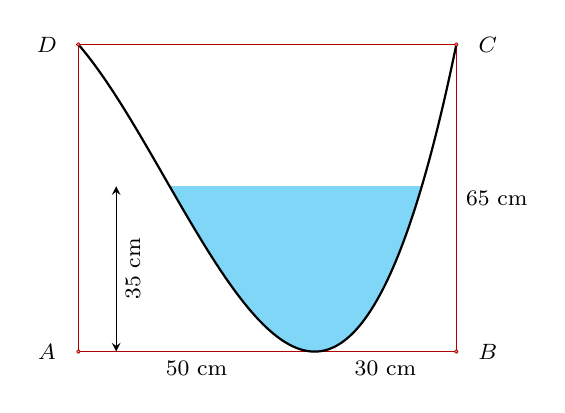
\begin{tikzpicture}[declare function={rong=8; h=6.5; mucnuoc=3.5; rong1=5; rong2=3; f(\x) = (13/225)*\x^3 - (143/450)*\x^2 - (52/45)*\x;},x=1cm,y=1cm,every node/.style={font=\footnotesize},line join=round,line cap=round,>=stealth,scale=0.6]
			\path
			(0,0) coordinate (D)
			(rong,0) coordinate (C)
			(rong,-h) coordinate (B)
			(0,-h) coordinate (A);
			\begin{scope}
				\clip (0,-h) rectangle (rong,-h+mucnuoc);
				\fill[cyan!50!white] plot[domain=0:rong,samples=500,smooth] (\x,{f (\x)}) -- (rong,0) -- (0,0) -- cycle;
			\end{scope}
			\draw[color=red!70!black] (A) -- (B) -- (C) -- (D) -- cycle;
			\draw[thick,color=black,smooth,samples=150,domain=0:rong] plot (\x,{f (\x)});
			\draw[<->] (0.8,-h) -- (0.8,-h+mucnuoc) node[pos=0.5,sloped,below] {$35$ cm};
			\path (rong1/2,-h) node[below] {$50$ cm};
			\path (rong1 + rong2/2,-h) node[below] {$30$ cm};
			\path (rong,-h/2) node[right] {$65$ cm};
			\foreach \p/\pos in {A/180,B/0,C/0,D/180}{
				\shade[ball color=red] (\p) circle (1.2pt) node[shift={(\pos:4mm)}] {$\p$};
			}
		\end{tikzpicture}
	}
	\loigiai{
		\begin{itemchoice}
			\itemch \immini{Chọn hệ trục tọa độ $Oxy$ với gốc $O\equiv D(0;0)$. Trục $Ox$ hướng theo vectơ $\overrightarrow{DC}$ nên $C$ nằm trên tia $Ox$.\\
				Vì chiều rộng hình chữ nhật là $AB=50+30=80$ cm nên $DC=80$ cm, suy ra $C(80;0)$.\\
				Trục $Oy$ hướng theo vectơ $\overrightarrow{AD}$ (từ dưới lên trên). Do đó, các điểm $A$, $B$ nằm ở phía dưới trục hoành nên có tung độ âm. \\
				Vì $AD=BC=65$ cm nên $A(0;-65)$ và $B(80;-65)$.
			}{
				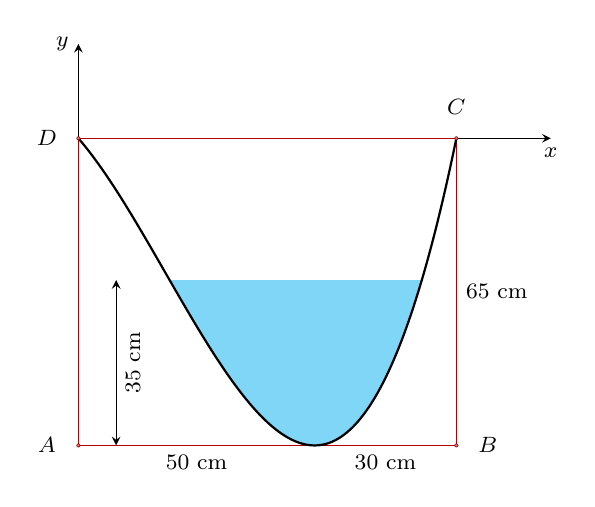
\begin{tikzpicture}[declare function={rong=8; h=6.5; mucnuoc=3.5; rong1=5; rong2=3; f (\x) = (13/225)*\x^3 - (143/450)*\x^2 - (52/45)*\x;},x=1cm,y=1cm,every node/.style={font=\footnotesize},line join=round,line cap=round,>=stealth,scale=0.6]
					\path
					(0,0) coordinate (D)
					(rong,0) coordinate (C)
					(rong,-h) coordinate (B)
					(0,-h) coordinate (A);
					\begin{scope}
						\clip (0,-h) rectangle (rong,-h+mucnuoc);
						\fill[cyan!50!white] plot[domain=0:rong,samples=500,smooth] (\x,{f (\x)}) -- (rong,0) -- (0,0) -- cycle;
					\end{scope}
					\draw[->] (D)--++(0,2) node[left] {$y$};
					\draw[->] (C)--++(2,0) node[below] {$x$};
					\draw[color=red!70!black] (A) -- (B) -- (C) -- (D) -- cycle;
					\draw[thick,color=black,smooth,samples=150,domain=0:rong] plot (\x,{f (\x)});
					\draw[<->] (0.8,-h) -- (0.8,-h+mucnuoc) node[pos=0.5,sloped,below] {$35$ cm};
					\path (rong1/2,-h) node[below] {$50$ cm};
					\path (rong1 + rong2/2,-h) node[below] {$30$ cm};
					\path (rong,-h/2) node[right] {$65$ cm};
					\foreach \p/\pos in {A/180,B/0,C/90,D/180}{
						\shade[ball color=red] (\p) circle (1.2pt) node[shift={(\pos:4mm)}] {$\p$};
					}
			\end{tikzpicture}}
			\itemch
			Theo hình vẽ, độ sâu của mực nước là $35$ cm (tính từ đáy $AB$ có tung độ $y=-65$). \\
			Do đó, phương trình biểu diễn mặt thoáng mực nước là $y=-65+35=-30$.
			\itemch Giả sử hàm số bậc ba có dạng $y=f(x)=ax^3+bx^2+cx+d$.
			\begin{itemize}
				\item Đồ thị đi qua $D(0;0)\Rightarrow d=0$.
				\item Đồ thị đi qua $C(80;0)\Rightarrow 80^3a+80^2b+80c=0\Leftrightarrow 6\,400a+80b+c=0\quad(1)$.
				\item Dựa vào hình vẽ, điểm thấp nhất của mặt cắt (cực tiểu của đồ thị) nằm trên đoạn $AB$ tại vị trí cách $A$ một đoạn $50$ cm, tức là cực tiểu tại $x=50$, $y=-65$.\\
				Ta có $f(50)=-65\Leftrightarrow 125\,000a+2\,500b+50c=-65\quad(2)$.
				\item Ta có $f'(x)=3ax^2+2bx+c$.\\
				Tại điểm cực tiểu $x=50$, ta có $f'(50)=0\Leftrightarrow 7\,500a+100b+c=0\quad(3)$.
			\end{itemize}
			Từ $(1)$, $(2)$ và $(3)$ ta được
			\[\heva{&6\,400a + 80b + c = 0\\&125\,000a + 2\,500b + 50c = -65\\&7\,500a + 100b + c = 0}\Leftrightarrow\heva{&a = \dfrac{13}{22\,500}\\&b = -\dfrac{143}{4\,500}\\&c = -\dfrac{52}{45}.}\]
			Suy ra phương trình đường lõm là $f(x)=\dfrac{13}{22\,500}x^3-\dfrac{143}{4\,500}x^2-\dfrac{52}{45}x$.\\
			Phương trình hoành độ giao điểm $f(x)=-30$ là
			\[\dfrac{13}{22\,500}x^3 - \dfrac{143}{4\,500}x^2 - \dfrac{52}{45}x = -30 \Leftrightarrow 13x^3 - 715x^2 - 26\,000x + 675\,000 = 0.\]
			Vì bề rộng mặt thoáng nằm trong đoạn $DC$ nên $x>0$, giải phương trình trên ta được $x_1\approx 19{,}31$ và $x_2\approx 72{,}69$.\\
			Bề rộng mặt thoáng là $d=x_2-x_1\approx 72{,}69-19{,}31=53{,}38$ cm $\neq 68{,}5$ cm.
			
			\itemch Diện tích mặt cắt của nước trong cối là phần diện tích giới hạn bởi đường thẳng $y=-30$ và đường cong $y=f(x)$, ta được
			\[S = \displaystyle\int\limits_{x_1}^{x_2} \bigg[-30 - f(x) \bigg] \mathrm{\,d}x = \displaystyle\int\limits_{19{,}31}^{72{,}69} \left( -30 - \dfrac{13}{22\,500}x^3 + \dfrac{143}{4\,500}x^2 + \dfrac{52}{45}x \right) \mathrm{\,d}x\approx 1\,214 \text{ cm}^2 \neq 1\,800 \text{ cm}^2.\]
		\end{itemchoice}
	}
\end{ex}
%%%=============================%%%

%%%=============EX_15=============%%%
\begin{ex}%[2D4V2-6]%[TDMZZ10]%[Nguyễn Văn Sang]
	Một ôtô được coi như một hạt chuyển động thẳng trên một đoạn đường. Ở thời điểm ban đầu ($t_0=0$) ôtô ở điểm $A$, đang chuyển động với biểu thức vận tốc $v_I = 1{,}2t + 10$ (m/s). Sau khi chuyển động được $12$ giây ôtô cách điểm $B$ trước mặt là $100$ m thì tài xế đạp phanh và bắt đầu giảm tốc độ với biểu thức vận tốc là $v_{II} = -2t + b$ (m/s). Khi vượt qua $B$ được $20$ m tài xế tăng tốc với biểu thức vận tốc $v_{III} = 2t + c$ (m/s), đến khi đạt được tốc độ $26$ m/s thì giữ tốc độ ổn định chuyển động thẳng đều.
	\begin{center}
		\begin{tikzpicture}[>=stealth, scale=0.95, font=\scriptsize, line cap=round, line join=round]
			\definecolor{carbody}{RGB}{220,30,30}
			\definecolor{darkcar}{RGB}{180,20,20}
			\definecolor{winblue}{RGB}{180,220,250}
			\definecolor{roadgray}{RGB}{140,140,140}
			
			\newcommand{\drawcar}[2]{
				\begin{scope}[shift={(#1,0)}, scale=0.4]
					\draw[fill=black] (-1.2,0.2) rectangle (1.2,0.4);
					\fill[black] (-0.8,0.2) circle (0.3);
					\fill[gray!50] (-0.8,0.2) circle (0.15);
					\fill[black] (0.9,0.2) circle (0.3);
					\fill[gray!50] (0.9,0.2) circle (0.15);
					\draw[fill=carbody, draw=darkcar] (-1.6,0.3) .. controls (-1.7,0.4) and (-1.7,0.7) .. (-1.5,0.8) -- (1.4,0.8) .. controls (1.6,0.7) and (1.6,0.4) .. (1.5,0.3) -- cycle;
					\draw[fill=carbody, draw=darkcar] (-1.0,0.8) .. controls (-0.8,1.3) .. (-0.4,1.4) -- (0.3,1.4) .. controls (0.7,1.3) .. (0.9,0.8) -- cycle;
					\draw[fill=winblue, draw=black!50] (-0.8,0.85) .. controls (-0.6,1.2) .. (-0.4,1.3) -- (-0.05,1.3) -- (-0.05,0.85) -- cycle;
					\draw[fill=winblue, draw=black!50] (0.05,0.85) -- (0.05,1.3) -- (0.3,1.3) .. controls (0.5,1.2) .. (0.7,0.85) -- cycle;
					\fill[yellow] (1.45,0.6) circle (0.08); 
					\ifnum#2=1 
					\foreach \y in {0.4, 0.6, 0.8} {
						\draw[blue!60, thick] (-1.8,\y) -- (-2.4,\y);
						\draw[blue!60, thick] (-1.9,\y+0.1) -- (-2.2,\y+0.1);
					}
					\fi
					\ifnum#2=2 
					\fill[red] (-1.6,0.6) circle (0.15);
					\shade[inner color=red, outer color=transparent] (-2.2,0.6) ellipse (0.8 and 0.4);
					\draw[red!50!white, thick] (-1.7,0.6) -- (-2.5,0.6);
					\draw[red!50!white, thick] (-1.65,0.7) -- (-2.3,0.7);
					\draw[red!50!white, thick] (-1.65,0.5) -- (-2.3,0.5);
					\fi
				\end{scope}
			}
			
			\fill[roadgray] (-1.5,-0.3) rectangle (15.5,0.3);
			\fill[black!80] (-1.5,0.3) rectangle (15.5,0.4); 
			\fill[black!80] (-1.5,-0.3) rectangle (15.5,-0.4); 
			
			\foreach \x in {-1,0,...,14} {
				\fill[white] (\x,-0.05) rectangle (\x+0.6,0.05);
			}
			
			\draw[dashed, blue!80!black, thick] (0, -2.4) -- (0, 4);
			\draw[dashed, blue!80!black, thick] (6, -2.4) -- (6, 4);
			\draw[dashed, blue!80!black, thick] (11.5, -2.4) -- (11.5, 4);
			\draw[dashed, blue!80!black, thick] (15, -2.4) -- (15, 4);
			
			\node[ align=center] at (3, 3.6) {Đoạn 1:\\Tăng tốc từ A};
			\node[ align=center] at (8.75, 3.6) {Đoạn 2:\\Phanh trước B};
			\node[ align=center] at (13.25, 3.6) {Đoạn 3:\\Tăng tốc sau B};
			
			\node[draw=black!20, fill=white, rounded corners, inner sep=2pt] at (3, 2.7) {$v(t) = 1{,}2t + 10\text{ (m/s)}$};
			\node[draw=black!20, fill=white, rounded corners, inner sep=2pt] at (8.75, 2.7) {$v(t) = -2t + b\text{ (m/s)}$};
			\node[draw=black!20, fill=white, rounded corners, inner sep=2pt] at (13.25, 2.7) {$v(t) = 2t + c\text{ (m/s)}$};
			
			\draw[->, line width=2pt, green!60!black] (2,1.8) -- (4,1.8) node[midway, above] {$v > 0$};
			\draw[->, line width=2pt, green!60!black] (7.75,1.8) -- (9.75,1.8) node[midway, above] {$v > 0$};
			\draw[->, line width=2pt, green!60!black] (12.25,1.8) -- (14.25,1.8) node[midway, above] {$v > 0$};
			
			\node[circle, fill=black, text=white, font=\bfseries\normalsize, inner sep=2pt] at (0,0) {A};
			\node[circle, fill=black, text=white, font=\bfseries\normalsize, inner sep=2pt] at (11.5,0) {B};
			
			\drawcar{3}{1}   
			\drawcar{8.75}{2} 
			\drawcar{13.25}{1}   
			
			\draw[->, thick] (5.2, 0.8) -- (5.8, 0.8);
			\draw[->, thick] (5.2, 0.4) -- (5.8, 0.4);
			
			\draw[->, line width=1.5pt, green!60!black] (1.5,-0.6) -- (4.5,-0.6) node[midway, below, align=center, text=black] {\bfseries Gia tốc\\$a = 1{,}2\text{ m/s}^2$};
			\draw[<-, line width=1.5pt, red] (7.5,-0.6) -- (10.5,-0.6) node[midway, below, align=center, text=black] {\bfseries Giảm tốc\\$a = -2\text{ m/s}^2$};
			\draw[->, line width=1.5pt, green!60!black] (12.8,-0.6) -- (14.5,-0.6) node[midway, below, align=center, text=black] {\bfseries Gia tốc\\$a = 2\text{ m/s}^2$};
			
			\node[fill=white,  align=center, inner sep=1pt] at (6.7, -1.0) {100m\\trước B};
			\node[fill=white,  align=center, inner sep=1pt] at (12.1, -1.0) {20m\\sau B};
			
			\draw[<->, thick] (6,-2.0) -- (11.5,-2.0) node[midway, fill=white, inner sep=2pt] { Khoảng cách = 100m};
			\draw[<->, thick] (11.5,-2.0) -- (15,-2.0) node[midway, fill=white, inner sep=2pt, align=center] { Khoảng cách = 20m};
			
			\draw[->, thick, gray!80!black] (0,-2.8) -- (15.5,-2.8) node[midway, below, text=black] { Thời gian $t$};
		\end{tikzpicture}
	\end{center}
	Hỏi trong các mệnh đề dưới đây, mệnh đề nào \textbf{đúng}, mệnh đề nào \textbf{sai}?
	\choiceTF
	{\True Vận tốc của vật ở thời điểm ban đầu bằng $10\text{ m/s}$}
	{$AB = 206{,}4\text{ m}$}
	{Tốc độ của vật tại $B$ là $3{,}6\text{ m/s}$ (làm tròn kết quả đến hàng phần mười)}
	{$c = -22{,}6$ (m/s)}
	\loigiai{
		\begin{itemchoice}
			\itemch Tại $t=0$, vận tốc ban đầu nằm ở đoạn 1: $v_I(0) = 1{,}2(0) + 10 = 10\text{ m/s}$.
			\itemch Sau $12\text{ s}$ đầu (kết thúc đoạn 1), quãng đường xe đi được là
			\[ s_1 = \displaystyle\int_{0}^{12} (1{,}2t+10) \mathrm{\,d}t = 206{,}4\text{ m}. \]
			Tại thời điểm này xe bắt đầu phanh và khoảng cách đến $B$ là $100\text{ m}$.\\
			Vậy tổng quãng đường từ $A$ đến $B$ là $AB = s_1 + 100 = 206{,}4 + 100 = 306{,}4\text{ m}$.
			\itemch Vận tốc tại thời điểm kết thúc đoạn 1 ($t=12\text{ s}$)
			\[ v_{12} = 1{,}2(12)+10 = 24{,}4\text{ m/s}. \]
			Đây cũng là vận tốc ban đầu của đoạn $2$. Trong giai đoạn $2$ (phanh), gia tốc $a_2 = -2\text{ m/s}^2$ (từ hàm $v_{II}$). Quãng đường từ lúc phanh đến điểm $B$ là $s = 100\text{ m}$.\\
			Áp dụng công thức độc lập, vận tốc tại $B$ ($v_B$)
			\[ v_B^2 - v_{12}^2 = 2a_2s \Rightarrow v_B^2 - (24{,}4)^2 = 2(-2)(100) = -400. \]
			\[ \Rightarrow v_B^2 = 595{,}36 - 400 = 195{,}36 \Rightarrow v_B = \sqrt{195{,}36} \approx 14{,}0\text{ m/s}. \]
			\itemch Đoạn 2 kết thúc khi vượt qua $B$ được $20\text{ m}$, tức là tổng quãng đường đoạn 2 là $s_2 = 100 + 20 = 120\text{ m}$.\\
			Vận tốc tại cuối đoạn 2 (gọi là $v_\text{cuối}$)
			\[ v_\text{cuối}^2 - (24{,}4)^2 = 2\cdot(-2)\cdot(120) = -480 \Rightarrow v_\text{cuối}^2 = 595{,}36 - 480 = 115{,}36. \]
			\[ \Rightarrow v_\text{cuối} = \sqrt{115{,}36} \approx 10{,}74\text{ m/s}. \]
			Từ hàm $v_{II}(t) = -2t + b$. Vận tốc liên tục tại $t=12$
			\[ v_{II}(12) = v_{12} \Rightarrow -2\cdot(12) + b = 24{,}4 \Rightarrow b = 48{,}4. \]
			Tại thời điểm $t_2$ kết thúc đoạn $2$
			\[ v_{II}(t_2) = v_\text{cuối} \Rightarrow -2t_2 + 48{,}4 = 10{,}74 \Rightarrow 2t_2 \approx 37{,}66 \Rightarrow t_2 \approx 18{,}83\text{ s}. \]
			Hàm vận tốc đoạn 3 là $v_{III}(t) = 2t + c$. Do vận tốc liên tục tại $t_2$
			\[ v_{III}(t_2) = v_\text{cuối} \Rightarrow 2(18{,}83) + c = 10{,}74 \Rightarrow 37{,}66 + c = 10{,}74 \Rightarrow c = -26{,}92. \]
		\end{itemchoice}
	}
\end{ex}
%%%=============================%%%

%%%=============EX_16=============%%%
\begin{ex}%[2D6V1-2]%[TDMZZ10]%[Hà Văn Hảo]
	Một công ty X có sản xuất $10\,000$ sản phẩm một loại mặt hàng Y. Công ty X giao cho ba xí nghiệp sản xuất: xí nghiệp $X_1$ sản xuất $5\,000$ sản phẩm ($X_1$ cho $200$ phế phẩm), xí nghiệp $X_2$ sản xuất $3\,000$ sản phẩm ($X_2$ cho $54$ phế phẩm), xí nghiệp $X_3$ sản xuất còn lại. Biết tổng phế phẩm trong $10\,000$ sản phẩm của ba xí nghiệp sản xuất là $290$. Chọn ngẫu nhiên một sản phẩm từ $10\,000$ sản phẩm loại mặt hàng Y. Gọi $A$ là biến cố \lq\lq chọn được sản phẩm của xí nghiệp $X_1$\rq\rq và $B$ là biến cố \lq\lq chọn được phế phẩm\rq\rq. Hỏi mệnh đề nào dưới đây là đúng hay sai?
	\choiceTF
	{\True $\mathrm{P}(A) = 0{,}5$}
	{\True Tỉ lệ phế phẩm của xí nghiệp $X_3$ là $1{,}8\,\%$}
	{$\mathrm{P}(\overline{A} \mid B) = \dfrac{1}{8}$}
	{$\mathrm{P}(B \mid \overline{A}) = \dfrac{2}{25}$}
	\loigiai{
		\begin{itemchoice}
			\itemch Tổng số sản phẩm là $10\,000$. Xí nghiệp $X_1$ sản xuất $5\,000$ sản phẩm.\\
			Xác suất chọn được sản phẩm của xí nghiệp $X_1$ là
			\[\mathrm{P}(A) = \dfrac{5\,000}{10\,000} = 0{,}5.\]
			\itemch Số sản phẩm xí nghiệp $X_3$ sản xuất là $10\,000 - (5\,000 + 3\,000) = 2\,000$ sản phẩm.\\
			Số phế phẩm của xí nghiệp $X_3$ là $290 - (200 + 54) = 36$ phế phẩm.\\
			Tỉ lệ phế phẩm của xí nghiệp $X_3$ là
			\[\dfrac{36}{2\,000} = 0{,}018 = 1{,}8\,\%.\]
			\itemch Biến cố $\overline{A}$ là biến cố \lq\lq chọn được sản phẩm không thuộc xí nghiệp $X_1$\rq\rq (tức là thuộc $X_2$ hoặc $X_3$).\\
			Số phế phẩm không thuộc xí nghiệp $X_1$ là $54 + 36 = 90$ phế phẩm.\\
			Tổng số phế phẩm là $n(B) = 290$.\\
			Xác suất có điều kiện $\mathrm{P}(\overline{A} \mid B)$ là xác suất chọn được sản phẩm của $X_2$ hoặc $X_3$ với điều kiện đó là phế phẩm
			\[\mathrm{P}(\overline{A} \mid B) = \dfrac{n(\overline{A} \cap B)}{n(B)} = \dfrac{90}{290} = \dfrac{9}{29}.\]
			\itemch Số sản phẩm không thuộc xí nghiệp $X_1$ là $n(\overline{A}) = 10\,000 - 5\,000 = 5\,000$ sản phẩm.\\
			Số phế phẩm trong nhóm này là $n(B \cap \overline{A}) = 90$.\\
			Xác suất có điều kiện $\mathrm{P}(B \mid \overline{A})$ là
			\[\mathrm{P}(B \mid \overline{A}) = \dfrac{n(B \cap \overline{A})}{n(\overline{A})} = \dfrac{90}{5\,000} = \dfrac{9}{500}.\]
		\end{itemchoice}
	}
\end{ex}
%%%=============================%%%
\caukq
%%%=============EX_17=============%%%
\begin{ex}%[2H5V1-7]%[TDMZZ10]%[Dương Công Tạo]
	Trong không gian $Oxyz$ có đơn vị dài trên mỗi trục là mét. Một ngôi nhà được lợp mái và hai mái nhà tầng hai đối xứng với nhau, có sàn nhà thuộc mặt phẳng $(Oxy)$, một mái nhà thuộc mặt phẳng $(\alpha) \colon x+19y+50z-100=0$, chiều rộng của một mái nhà là $3{,}2$ mét, độ cao của ngôi nhà là $9$ mét. Hãy xác định theo đơn vị mét độ cao của điểm thấp nhất trên mái nhà so với sàn nhà (\textit{làm tròn kết quả đến hàng phần trăm})?
	\begin{center}
		%%%%% Ngôi nhà
		\begin{tikzpicture}[scale=.7, >=stealth, line join=round, line cap=round, font=\footnotesize]
			\path (0,0) coordinate (o)
			++(10:2.5) coordinate (a)
			++(180:6.5) coordinate (b)
			++($(o)-(a)$) coordinate (c)
			\foreach \x in {o,b,c}{
				(\x)++(90:3) coordinate (\x')
			}
			(a)++(90:3.05) coordinate (a')
			(o')++(0:.3) coordinate (A)
			++(60:2) coordinate (O)
			(a)++(90:3)++(0:.3) coordinate (B)
			(o')++(60:2) coordinate (a1)
			(c')++(180:.3) coordinate (c1)
			(O)++($(c1)-(A)$) coordinate (O1)
			(B)++($(c1)-(A)$) coordinate (B1)
			;
			\fill [red!50!black!90] (O)--(B)--(B1)--(O1)--cycle;
			\fill [white] (o)--(o')--(a1)--(a')--(a)--cycle;
			\fill [pattern=horizontal lines] (o)--(o')--(c')--(c)--cycle;
			\fill [pattern=crosshatch dots] (o)--(o')--(a1)--(a')--(a)--cycle;
			\fill [red!70!black!90] (c1)--(O1)--(O)--(A)--cycle;
			\foreach \x in {1,2,3,4,5,6,7,8,9}{
				\foreach \y in {0,2,4}{
					\draw [thick, black!70] ($(O)!\x/10!(O1)+(O1)!\y/6!(c1)-(O1)$)--++($(O1)!1/6!(c1)-(O1)$);
				}
			}
			\foreach \x in {.5,1.5,...,9.5}{
				\foreach \y in {1,3,5}{
					\draw [thick, black!70] ($(O)!\x/10!(O1)+(O1)!\y/6!(c1)-(O1)$)--++($(O1)!1/6!(c1)-(O1)$);
				}
			}
			\foreach \x in {1,2,3,4,5}{
				\draw [thick, black!70] ($(O1)!\x/6!(c1)$)--++($(A)-(c1)$);
			}
			\foreach \x in {0,1}{
				\fill[white] ({-1-2*\x*1.5},.75) rectangle ++(-1.5,1.5);
				\fill ({-1.4-2*\x*1.5},.8) rectangle ++(-.7,1.3);
				\draw [thick, white] ({-1.6-2*\x*1.5},.8)--++(90:1.3)
				({-1.9-2*\x*1.5},.8)--++(90:1.3)
				({-1.4-2*\x*1.5},1)--++(180:.7)
				({-1.4-2*\x*1.5},1.45)--++(180:.7)
				({-1.4-2*\x*1.5},1.9)--++(180:.7);
			}
			\fill [white] (o)++(.5,.75)--++(90:1.5)--++(10:1.5)--++(-90:1.5)--cycle;
			\fill (o)++(.5,.85)++(10:.4)--++(90:1.3)--++(10:.7)--++(-90:1.3)--cycle;
			\draw [thick, white] (o)++(.5,.85)++(10:.6)--++(90:1.3)
			(o)++(.5,.85)++(10:.9)--++(90:1.3)
			(o)++(.5,1.05)--++(10:1.3)
			(o)++(.5,1.5)--++(10:1.3)
			(o)++(.5,1.95)--++(10:1.3)
			;
			\draw [thick] (c')--(c)--(o) (o')--(o)--(a)--(a') (O)--(O1)--(c1)--(A)--cycle (B)--++(180:.3);
		\end{tikzpicture}
		\hspace*{2cm}
		\begin{tikzpicture}[scale=0.7, >=stealth, line join=round, line cap=round, font=\footnotesize]
			\path
			(0,0) coordinate (O)
			+(0:.25) coordinate (j)
			+(-130:.4) coordinate (i)
			+(90:.5) coordinate (k)
			\foreach \l/\x/\y/\z in {A/0/0, B/10/0/0, C/10/16/0, D/0/16/0, E/0/0/7.86, F/10/0/7, G/10/16/7, H/00/16/7.86, I/10/8/9, K/0/8/9, I'/10/8/0}{
				($\x*(i)+\y*(j)+\z*(k)$) coordinate (\l)
			}
			;
			\draw[dash pattern=on 1.5pt off 1.5pt] (B)--(A)--(D) (A)--(E)--(H);
			\draw[semithick] (B)--(C)--(D) (E)--(F)--(G)--(H) (B)--(F) (C)--(G) (D)--(H) (F)--(I)--(G) (E)--(K)--(H) (I)--(K);
			\foreach \x in {O, B, C, D, E, F, G, H, I, K, I'}{
				\draw[fill=black] (\x) circle (1pt);
			}
		\end{tikzpicture}
	\end{center}
	\shortans[oly]{7{,}86}
	\loigiai{
		Xét mặt cắt ngôi nhà như hình vẽ dưới đây
		\begin{center}
			\begin{tikzpicture}[scale=0.5, >=stealth, line join=round, line cap=round, font=\footnotesize]
				\path (0,0) coordinate (A)
				++(0:10) coordinate (B)
				++(90:7.86) coordinate (C)
				++($(A)-(B)$) coordinate (D)
				($(A)!.5!(B)$) coordinate (I)
				++(90:9) coordinate (E)
				($(C)!.5!(D)$) coordinate (K)
				;
				\draw [semithick] (A)--(B)--(C)--(D)--cycle
				(C)--(E) node [above, pos=.5, sloped] {$3{,}2$ m}--(D)
				(E)--(I)
				;
				\pic [draw, angle radius=0.15cm] {right angle=C--K--E};
				\pic [draw, angle radius=0.15cm] {right angle=B--I--K};
				\draw [dash pattern=on 1.5pt off 1.5pt] (E)--++(180:7)
				(A)--++(180:2);
				\draw [<->] (E)++(180:7)--++($(I)-(E)$) node [pos=.5, sloped, fill=white] {$9$ m};
				\foreach \x/\y in {A/-90, B/-90, D/180, C/0, I/-90, K/-135, E/90}{
					\draw[fill=black] (\x) circle (1pt) ++(\y:0.6) node {$\x$};
				}
			\end{tikzpicture}
		\end{center}
		Khi đó, chiều cao ngôi nhà là $EI=9$\,m, chiều rộng mái nhà là $CE=3{,}2$\,m. \\
		Góc $ECK$ là góc giữa mặt phẳng $(\alpha)$ (mặt phẳng chứa mái nhà) và mặt phẳng $(Oxy)$ (mặt sàn). \\
		Khoảng cách từ điểm thấp nhất trên mái nhà so với sàn là
		\[CB=KI=EI-EK.\]
		Mặt phẳng $(\alpha)$ có vectơ pháp tuyến $\overrightarrow{n}=(1;19;50)$, mặt phẳng $(Oxy)$ có vectơ pháp tuyến $\overrightarrow{k}=(0;0;1)$. \\
		Khi đó
		\[\cos\widehat{ECK}=\left|\cos\left(\overrightarrow{n},\overrightarrow{k}\right)\right|=\dfrac{|1 \cdot 0+19 \cdot 0+50 \cdot 1|}{\sqrt{1^2+19^2+50^2} \cdot \sqrt{0^2+0^2+1^2}}=\dfrac{50}{3\sqrt{318}}.\]
		$\Rightarrow \sin\widehat{ECK}=\sqrt{1-\cos^2\widehat{ECK}}=\sqrt{\dfrac{181}{1\,431}}$. \\
		Trong tam giác $EKC$ vuông tại $K$, ta có
		\[EK=EC \cdot \sin\widehat{ECK}=3{,}2 \cdot \sqrt{\dfrac{181}{1\,431}} \approx 1{,}138 \text{ (m)}.\]
		Vậy $CB=EI-EK \approx 9-1{,}138 \approx 7{,}86$\,m.
	}
\end{ex}
%%%=============================%%%

%%%=============EX_18=============%%%
\begin{ex}%[2H2V2-5]%[TDMZZ10]%[Vũ Hồng Toàn]
	Cho tứ diện $ABCD$ có $\mathrm{d}\left(A, CD\right) = 7$, $\mathrm{d}\left(B, CD\right) = 9$, $AB = 11$ và góc giữa hai đường thẳng $AB$ và $CD$ bằng $70^\circ$. Tính theo đơn vị độ số đo góc nhị diện $\left[A, CD, B\right]$ {\it (làm tròn kết quả đến hàng đơn vị)}.
	\shortans[oly]{79}
	\loigiai{
		Gọi $H$ và $K$ lần lượt là hình chiếu vuông góc của $A$ và $B$ lên đường thẳng $CD$. \\
		Khi đó $AH = \mathrm{d}\left(A, CD\right) = 7$ và $BK = \mathrm{d}\left(B, CD\right) = 9$. \\
		Gọi $\varphi$ là số đo góc nhị diện $\left[A, CD, B\right]$.\\
		Vì $AH \perp CD$ và $BK \perp CD$ nên $\varphi$ chính là góc giữa hai đường thẳng $AH$ và $BK$.\\
		Chọn hệ trục tọa độ ${Oxyz}$ sao cho
		\begin{itemize}
			\item Trục $Oz$ trùng với đường thẳng $CD$.
			\item Điểm $H$ trùng với gốc tọa độ $O(0; 0; 0)$.
			\item Điểm $A$ thuộc tia $Ox$, suy ra $A(7; 0; 0)$.
			\item Điểm $K$ nằm trên trục $Oz$, gọi tọa độ là $K(0; 0; c)$. Khi đó độ dài đoạn $HK = |c|$.
			\item Điểm $B$ có khoảng cách đến $CD$ bằng $9$ và mặt phẳng $(BCD)$ tạo với mặt phẳng $(ACD)$. Suy ra, tọa độ của $B\left(9 \cos \varphi; 9 \sin \varphi; c\right)$.
		\end{itemize}
		Tham khảo hình vẽ
		\begin{center}
			\begin{tikzpicture}[scale=1, font=\footnotesize, line join=round, line cap=round, >=stealth]
				\tikzset{declare function={h=2;b=h;goc=-130;a=1.5*h;}}
				\path (0:0) coordinate (H)coordinate (O)
				(goc:b) coordinate (A) (0,-h/2)coordinate (C)
				(40:b+1) coordinate (B)
				(a,0) coordinate (Ex)
				(intersection of C--B and H--Ex) coordinate (E)
				($(O)!(B)!(H)$) coordinate (K)++(0,h/2)coordinate (D);
				\draw[dashed]  (A)--(O)--(E)--(C)--cycle (C)--(D) (K)--(B);
				\draw (A)--(D)--(B)--(E);
				\draw[->] (E)--($(O)!3.5!(E)$)node[below]{$y$};
				\draw[->] (A)--($(O)!1.5!(A)$)node[right]{$x$};
				\draw[->] (D)--++(0,0.6)node[left]{$z$};
				\foreach \x/\y/\z in {B/K/H} \draw pic[draw,angle radius=2mm]{right angle= \x--\y--\z};
				\foreach \x /\gN in {A/160,B/0,C/-90,D/180,K/40,O/180,H/45}
				\fill (\x) circle (1pt)	($(\x)+(\gN:2.5mm)$) node {$\x$};
			\end{tikzpicture}
		\end{center}
		Ta có $\overrightarrow{AB} = \left(9 \cos \varphi - 7; 9 \sin \varphi; c\right)$.\\
		Suy ra
		\begin{align*}
			AB^2 &= (9 \cos \varphi - 7)^2 + (9 \sin \varphi)^2 + c^2\\
			\Leftrightarrow 11^2 &= 81 \cos^2 \varphi - 126 \cos \varphi + 49 + 81 \sin^2 \varphi + c^2\\
			\Leftrightarrow 11^2&=81(\cos^2 \varphi + \sin^2 \varphi) + 49 - 126 \cos \varphi + c^2\\
			\Leftrightarrow 121 &= 130 - 126 \cos \varphi + c^2.\qquad (1)
		\end{align*}
		Mặt khác, góc giữa $AB$ và $CD$ là $70^\circ$. Vectơ chỉ phương của $CD$ là $\overrightarrow{u} = (0; 0; 1)$.\\
		Ta có $\cos 70^\circ = \dfrac{|\overrightarrow{AB} \cdot \overrightarrow{u}|}{|\overrightarrow{AB}| \cdot |\overrightarrow{u}|} = \dfrac{|c|}{11 \cdot 1} \Rightarrow |c| = 11 \cos 70^\circ$.\\
		Suy ra $c^2 = \left(11 \cos 70^\circ\right)^2$.\qquad $(2)$\\
		Thay $(2)$ vào $(1)$, ta được
		\begin{align*}
			121 &= 130 - 126 \cos \varphi + 121 \cos^2 70^\circ\\
			\Leftrightarrow 126 \cos \varphi &= 9 + 121 \cos^2 70^\circ\\
			\Rightarrow \cos \varphi &= \dfrac{9 + 121 \cdot \cos^2 70^\circ}{126}\\
			\Rightarrow \varphi &\approx 79^\circ.
		\end{align*}
	}
\end{ex}
%%%=============================%%%

%%%=============EX_19=============%%%
\begin{ex}%[1H8V7-9]%[TDMZZ10]%[Duong Xuan Loi]
	\immini{
		Cho một bình ban đầu chưa đựng gì như hình vẽ. Bình có dạng hình lăng trụ đều với cạnh đáy bằng $60$ cm và cạnh bên bằng $90$ cm bên trong có một quả cầu đặc bán kính $20$ cm không thấm nước như hình vẽ. Ta tiến hành dùng một vòi nước cho chảy vào bình với lưu lượng không đổi bằng $L$ cm$^3$/phút. Biết rằng sau khoảng thời gian $120$ phút thì vòi chảy đầy bình. Hãy xác định theo đơn vị centimet độ cao của mực nước trong bình sau khi vòi nước chảy được $15$ phút (mặt nước so với đáy) (\textit{làm tròn kết quả đến hàng đơn vị})?
	}{
		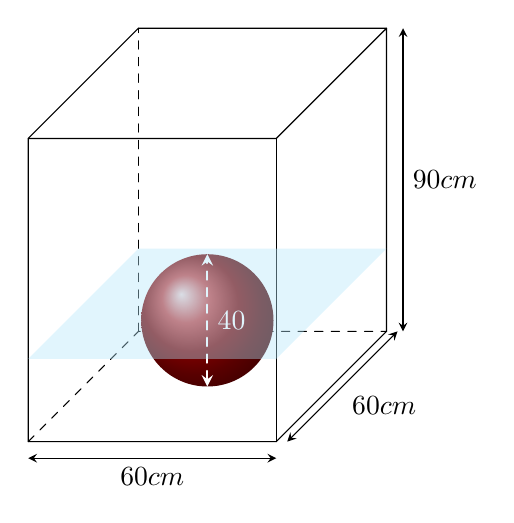
\begin{tikzpicture}[scale=0.7, line join=round, line cap=round, >=stealth]
			\def\a{4.5} 
			\def\b{2} 
			\def\h{5.5} 
			\coordinate (A) at (0,0);
			\coordinate (B) at (\a,0);
			\coordinate (C) at (\a+\b,\b);
			\coordinate (D) at (\b,\b);
			\coordinate (A') at (0,\h);
			\coordinate (B') at (\a,\h);
			\coordinate (C') at (\a+\b,\b+\h);
			\coordinate (D') at (\b,\b+\h);
			\draw[dashed] (A) -- (D) -- (C);
			\draw[dashed] (D) -- (D');
			\coordinate (center) at (\a/2+\b/2, \b/2 + 1.2);
			\shade[ball color=red!70!black] (center) circle (1.2);
			\draw[<->, dashed, white, thick] (\a/2+\b/2, \b/2) -- (\a/2+\b/2, \b/2 + 2.4) node[midway, right] {40};
			\draw (A) -- (B) -- (C) -- (C') -- (B') -- (A') -- cycle;
			\draw (B) -- (B');
			\draw (A') -- (D') -- (C');
			\draw[<->] (0,-0.3) -- (\a,-0.3) node[midway, below] {$60\text{ cm}$};
			\draw[<->] (\a+0.2,0) -- (\a+\b+0.2,\b) node[midway, below right] {$60\text{ cm}$};
			\draw[<->] (\a+\b+0.3,\b) -- (\a+\b+0.3,\b+\h) node[midway, right] {$90\text{ cm}$};
			\def\wh{1.5}
			\fill[cyan!30, opacity=0.4] (0,\wh) -- (\a,\wh) -- (\a+\b,\b+\wh) -- (\b,\b+\wh) -- cycle;
		\end{tikzpicture}
	}
	\shortans{$12$}
	\loigiai{
		Thể tích của bình khi không đựng gì là $V_b = 60^2 \cdot 90 = 324\,000\text{ (cm}^3\text{)}$.\\
		Thể tích của quả cầu đặc là $V_c = \dfrac{4}{3}\pi R^3 = \dfrac{4}{3}\pi \cdot 20^3 = \dfrac{32\,000\pi}{3}\text{ (cm}^3\text{)}$.\\
		Thể tích nước cần thiết để làm đầy bình là $V_1 = V_b - V_c = 324\,000 - \dfrac{32\,000\pi}{3}\text{ (cm}^3\text{)}$.\\
		Gọi $V_2$ là thể tích nước để vừa ngập quả bóng $V_2=60^2\cdot 40-V_c=60^2\cdot40-\dfrac{4\pi}{3}\cdot20^3$.\\
		Lưu lượng nước chảy vào bình mỗi phút là $L = \dfrac{V_1}{120} = \dfrac{324\,000 - \dfrac{32\,000\pi}{3}}{120} = 2\,700 - \dfrac{800\pi}{9}\text{ (cm}^3/\text{phút)}$.\\
		Thể tích nước chảy vào bình sau $15$ phút là $V_{15} = 15L = 15\left(2\,700 - \dfrac{800\pi}{9}\right) = 40\,500 - \dfrac{4\,000\pi}{3}\text{ (cm}^3\text{)}$.\\
		Ta thấy $V_{15}<V_2$ nên sau $15$ phút nước chưa ngập quả bóng.\\
		Gọi $h\text{ (cm)}$ ($0 < h < 40$) là độ cao của mực nước trong bình sau $15$ phút.\\
		Thể tích nước $V_{15}$ bằng thể tích khối hộp chữ nhật có chiều cao $h$ trừ đi phần thể tích chỏm cầu bị ngập trong nước.\\
		Thể tích khối hộp chữ nhật có độ cao $h$ là $V_h = 60^2 \cdot h = 3\,600h$.\\
		Thể tích chỏm cầu (bán kính $R=20$) bị ngập nước có chiều cao $h$ là
		\[V_{ch} = \pi h^2 \left( R - \dfrac{h}{3} \right) = \pi h^2 \left( 20 - \dfrac{h}{3} \right) = 20\pi h^2 - \dfrac{\pi}{3}h^3.\]
		Ta có phương trình
		\[3\,600h - \left( 20\pi h^2 - \dfrac{\pi}{3}h^3 \right) = 40\,500 - \dfrac{4\,000\pi}{3} \Leftrightarrow \dfrac{\pi}{3}h^3 - 20\pi h^2 + 3\,600h - 40\,500 + \dfrac{4\,000\pi}{3} = 0\Leftrightarrow h\approx 12.\]
		Vậy độ cao mực nước xấp xỉ $12$\,cm.
	}
\end{ex}
%%%=============================%%%

%%%=============EX_20=============%%%
\begin{ex}%[0D8V1-3]%[TDMZZ10]%[Lê Hồ Quang Minh]
	Dùng $5$ màu sắc khác nhau: đỏ, cam, vàng, lục, tím để tô màu cho $8$ ô vuông nhỏ trong hình vẽ, mỗi ô vuông được tô đúng một màu. Hai cách tô màu được gọi là
	khác nhau nếu ta xếp $8$ ô vuông theo một thứ tự nào đó thì có ít nhất một vị trí cho màu khác nhau. Gọi $T$ là số cách tô thoả mãn đồng thời hai điều kiện
	\begin{itemize}
		\item Có đúng hai ô được tô màu cam.
		\item Các ô có chung cạnh được tô màu khác nhau.
	\end{itemize}
	\begin{center}
		
\begin{tikzpicture}[scale=1.5]
			\definecolor{mygreen}{RGB}{0, 176, 80}
			\definecolor{mypurple}{RGB}{112, 48, 160}
			\definecolor{myorange}{RGB}{255, 192, 0}
			\definecolor{myred}{RGB}{255, 0, 0}
			\definecolor{myyellow}{RGB}{255, 255, 0}
			\draw[fill=mygreen] (0,1) rectangle (1,2);
			\draw[fill=mypurple] (1,1) rectangle (2,2);
			\draw[fill=myorange] (2,1) rectangle (3,2);
			\draw[fill=mypurple] (3,1) rectangle (4,2);
			\draw[fill=mypurple] (0,0) rectangle (1,1);
			\draw[fill=myorange] (1,0) rectangle (2,1);
			\draw[fill=myred] (2,0) rectangle (3,1);
			\draw[fill=myyellow] (3,0) rectangle (4,1);
			\draw[red, thick] (0,0) grid (4,2);
			\draw[red, ultra thick] (0,0) rectangle (4,2);
		\end{tikzpicture}
	\end{center}
	Hãy tính $\dfrac{T}{21}$ \textit{(Làm tròn kết quả đến hàng đơn vị).}
	\shortans[oly]{830}
	\loigiai{
		Sử dụng điều kiện có đúng hai ô được tô màu cam, ta chia bài toán thành các trường hợp sau
		\begin{itemize}
			\item \textbf{Trường hợp 1:} Hai ô được tô màu cam ở cột $1$ và cột $2$ hoặc ở cột $3$ và cột $4$.
			
			Khi đó, số cách tô màu là $4 \cdot \left[(4-1)^4 + (4-1)\cdot (-1)^4\right]\cdot 3 \cdot 4 = 4\,032$.
			\item \textbf{Trường hợp 2:} Hai ô được tô màu cam ở cột $1$ và cột $3$ hoặc ở cột $2$ và cột $4$.
			
			Khi đó, số cách tô màu là $8 \cdot 4 \cdot 3^5 = 7\,776$.
			\item \textbf{Trường hợp 3:} Hai ô được tô màu cam ở cột $1$ và cột $4$.
			
			Khi đó, số cách tô màu là $4 \cdot \left[(4-1)^4 + (4-1)\cdot (-1)^4\right]\cdot 3 \cdot 3 = 3\,024$.
			\item \textbf{Trường hợp 4:} Hai ô được tô màu cam ở cột $2$ và cột $3$.
			
			Khi đó, số cách tô màu là $2 \cdot (4\cdot 3^2)\cdot (4 \cdot 3^2) = 2\,592$.
		\end{itemize}
		Suy ra số cách tô màu thỏa mãn hai điều kiện của bài toán là $$T = 4\,032 + 7\,776 + 3\,024 + 2\,592 = 17\,424.$$
		Vậy $\dfrac{T}{21} \approx 830$.
	}
\end{ex}
%%%=============================%%%

%%%=============EX_21=============%%%
\begin{ex}%[2D4V3-2]%[TDMZZ10]%[Nguyễn Đức Tuấn Anh]
	\immini[thm]{
		Có một tờ giấy hình parabol có chiều cao bằng $60$ cm. Ta tiến hành gấp tờ giấy theo một đường nằm ngang song song với cạnh $AB$. Hãy tính giá trị nhỏ nhất của phần diện tích còn lại sau khi gấp so với diện tích ban đầu của tờ giấy (\textit{làm tròn kết quả đến hàng phần trăm})?}{
		\begin{tikzpicture}[scale=.7, font=\footnotesize, line join=round, line cap=round, >=stealth]
			\fill[cyan!15] (-3,0) -- plot[domain=-3:3, samples=100] (\x, {6 - (2/3)*(\x)*(\x)}) -- cycle;
			\draw[blue, thick] plot[domain=-3:3, samples=100] (\x, {6 - (2/3)*(\x)*(\x)});
			\draw[blue,thick] (-3,0) -- (3,0);
			\draw[dashed,thick] (-4.5, 2.2) -- (4.5, 2.2)node[pos=.9,above]{đường gấp};
			\node[below] at (-3, 0) {$A$};
			\node[below] at (3, 0) {$B$};
			\draw[dashed] (0, 6) -- (-4.5, 6) (-3, 0) -- (-4.5, 0);
			\draw[<->] (-4.2, 0) -- (-4.2, 6) node[midway, fill=white, inner sep=3pt] {$60$ cm};
		\end{tikzpicture}
	}
	\shortans{$0{,}62$}
	\loigiai{
		Chọn hệ trục tọa độ sao cho đỉnh parabol ban đầu là $I(0;60)$ và trục đối xứng là trục tung $Oy$.
		Phương trình của parabol ban đầu có dạng $y = 60 - ax^2$ ($a > 0$).\\
		Diện tích hình phẳng giới hạn bởi parabol $y = 60 - ax^2$ và đường thẳng $y = t$ ($0 \le t \le 60$) là
		\[ S(t) = 2\displaystyle\int\limits_0^{\sqrt{\frac{60-t}{a}}} \left(60 - t - ax^2\right) \mathrm{\,d}x = \dfrac{4}{3\sqrt{a}}(60 - t)^{\frac{3}{2}}. \]
		Từ đó, diện tích ban đầu của tờ giấy là
		\[ S_0 = S(0) = \dfrac{4}{3\sqrt{a}} 60^{\frac{3}{2}}. \]
		Giả sử ta gấp tờ giấy theo đường nằm ngang $y = t$ ($0 \le t \le 60$). Phần parabol phía trên đường $y=t$ bị gập xuống dưới có diện tích là $S_1 = S(t)$.
		\begin{center}
			\begin{tikzpicture}[line cap=round, line join=round, >=stealth, font=\footnotesize,scale=.9]
				\begin{scope}[shift={(0,0)}]
					\pgfmathsetmacro{\rtA}{sqrt(3)}
					\fill[cyan!15] (-3,0) -- plot[domain=-3:-\rtA, samples=40] (\x, {6-(2/3)*\x*\x}) -- (-\rtA,4) -- (\rtA,4) -- plot[domain=\rtA:3, samples=40] (\x, {6-(2/3)*\x*\x}) -- cycle;
					\fill[red!15, opacity=0.9] plot[domain=-\rtA:\rtA, samples=40] (\x, {2+(2/3)*\x*\x}) -- (\rtA,4) -- (-\rtA,4) -- cycle;
					\draw[->] (-4,0) -- (4.2,0) node[above] {$x$};
					\draw[->] (0,-1) -- (0,6.5) node[left] {$y$};
					\draw[thick] (-3,0) -- (3,0);
					\draw[thick] plot[domain=-3:-\rtA, samples=40] (\x, {6-(2/3)*\x*\x});
					\draw[thick] plot[domain=\rtA:3, samples=40] (\x, {6-(2/3)*\x*\x});
					\draw[thick, dashed, gray] plot[domain=-\rtA:\rtA, samples=40] (\x, {6-(2/3)*\x*\x});
					\draw[thick, red] plot[domain=-\rtA:\rtA, samples=40] (\x, {2+(2/3)*\x*\x});
					\draw[dashed, blue, thick] (-3.5,4) -- (3.5,4) node[right, black] {$y=t$};
					\foreach \px/\py/\anch/\lbl in {0/0/below left/O, -3/0/below left/A, 3/0/below right/B, 0/6/above right/I(0; 60), 0/2/below right/(0; 2t-60)}
					\fill (\px,\py) circle (1.5pt) node[\anch] {$\lbl$};
					\node[right] at (0,3.2) {$S_1$};
					\node[font=\bfseries] at (0,7.25) {Trường hợp 1: $30 \le t \le 60$};
				\end{scope}
				\begin{scope}[shift={(9,0)}]
					\pgfmathsetmacro{\rtB}{sqrt(6)}
					\pgfmathsetmacro{\rtC}{sqrt(3)}
					\fill[cyan!15] (-3,0) -- plot[domain=-3:-\rtB, samples=40] (\x, {6-(2/3)*\x*\x}) -- (-\rtB,2) -- (\rtB,2) -- plot[domain=\rtB:3, samples=40] (\x, {6-(2/3)*\x*\x}) -- cycle;
					\fill[red!15, opacity=0.9] plot[domain=-\rtB:\rtB, samples=50] (\x, {(2/3)*\x*\x-2}) -- (\rtB,2) -- (-\rtB,2) -- cycle;
					\fill[orange!40, opacity=0.9] plot[domain=-\rtC:\rtC, samples=40] (\x, {(2/3)*\x*\x-2}) -- (\rtC,0) -- (-\rtC,0) -- cycle;
					\draw (-4,0)--(3,0);
					\draw[->] (3,0) -- (4.2,0) node[above] {$x$};
					\draw[->] (0,-2.25) -- (0,6.5) node[left] {$y$};
					\draw[thick] (-3,0) -- (-\rtC,0) (\rtC,0) -- (3,0);
					\draw[thick, dashed, gray] (-\rtC,0) -- (\rtC,0);
					\draw[thick] plot[domain=-3:-\rtB, samples=40] (\x, {6-(2/3)*\x*\x});
					\draw[thick] plot[domain=\rtB:3, samples=40] (\x, {6-(2/3)*\x*\x});
					\draw[thick, dashed, gray] plot[domain=-\rtB:\rtB, samples=40] (\x, {6-(2/3)*\x*\x});
					\draw[thick, red] plot[domain=-\rtB:\rtB, samples=50] (\x, {(2/3)*\x*\x-2});
					\draw[dashed, blue, thick] (-3.5,2) -- (3.5,2) node[right, black] {$y=t$};
					\foreach \px/\py/\anch/\lbl in {0/0/below left/O, -3/0/below left/A, 3/0/below right/B, 0/6/above right/I(0; 60), 0/-2/below right/(0; 2t-60)}
					\fill (\px,\py) circle (1.5pt) node[\anch] {$\lbl$};
					\node[right] at (0,0.8) {$S_1$};
					\node[right] at (0,-0.8) {$S_2$};
					\node[font=\bfseries] at (0,7.25) {Trường hợp 2: $0 \le t < 30$};
				\end{scope}
			\end{tikzpicture}
		\end{center}
		\begin{enumerate}[\it TH 1:]
			\item $30 \le t \le 60$. \\
			Đỉnh của phần gấp xuống là $(0;2t - 60)$ có tung độ không âm nên phần gấp nằm hoàn toàn bên trong giới hạn của tờ giấy ban đầu.\\
			Khi đó, diện tích hình phẳng phần còn lại (phần nhìn thấy) là
			\[ S = S_0 - S_1 = S_0 - S_0 \left(\dfrac{60-t}{60}\right)^{\frac{3}{2}} = S_0 \left[ 1 - \left(1 - \dfrac{t}{60}\right)^{\frac{3}{2}} \right]. \]
			Do $t \ge 30$ nên tỉ số $\dfrac{S}{S_0}$ đạt giá trị nhỏ nhất tại $t = 30$, khi đó
			\[ \dfrac{S}{S_0} = 1 - \dfrac{1}{2\sqrt{2}} \approx 0{,}646. \]
			\item $0 \le t < 30$. \\
			Đỉnh của phần gấp xuống vươn ra khỏi mép dưới $AB$ (trục hoành).\\
			Phần nhô ra ngoài mép dưới tạo thành một hình parabol nhỏ có đỉnh $(0;2t - 60)$ và đường chuẩn là trục hoành.\\
			Diện tích của phần nhô ra này tương ứng với đoạn parabol có chiều cao $60-2t$, do đó có diện tích là
			\[ S_2 = S(2t) = \dfrac{4}{3\sqrt{a}}(60 - 2t)^{\frac{3}{2}} = S_0 \left(\dfrac{60-2t}{60}\right)^{\frac{3}{2}}. \]
			Diện tích hình phẳng phần còn lại bằng tổng diện tích phần không bị gấp đè và diện tích phần nhô ra
			\[ S = S_0 - S_1 + S_2 = S_0 \left[ 1 - \left(1 - \dfrac{t}{60}\right)^{\frac{3}{2}} + \left(1 - \dfrac{2t}{60}\right)^{\frac{3}{2}} \right]. \]
			Đặt $u = 1 - \dfrac{t}{60}$, vì $t \in [0;30)$ nên $u \in \left( \dfrac{1}{2}; 1 \right]$.\\
			Xét hàm số $f(u) = 1 - u^{\frac{3}{2}} + (2u - 1)^{\frac{3}{2}}$ trên $\left( \dfrac{1}{2}; 1 \right]$.
			Ta có
			\[ f'(u) = -\dfrac{3}{2}u^{\frac{1}{2}} + \dfrac{3}{2} \cdot 2(2u - 1)^{\frac{1}{2}} = \dfrac{3}{2} \left( 2\sqrt{2u - 1} - \sqrt{u} \right). \]
			Cho $f'(u) = 0 \Leftrightarrow 2\sqrt{2u - 1} = \sqrt{u} \Leftrightarrow 4(2u - 1) = u \Leftrightarrow u = \dfrac{4}{7}$ (thỏa mãn).\\
			Bảng biến thiên
			\begin{center}
				
\begin{tikzpicture}
					\tkzTabInit[lgt=1.5, espcl=4]
					{$u$ / 1, $f'(u)$ / 1, $f(u)$ / 2.5}
					{$\dfrac{1}{2}$, $\dfrac{4}{7}$, $1$}
					\tkzTabLine{ , -, z, +, }
					\tkzTabVar{ +/, -/$f\left(\dfrac{4}{7}\right)$, +/}
				\end{tikzpicture}
			\end{center}
			
			Do đó $f(u)$ đạt giá trị nhỏ nhất tại $u = \dfrac{4}{7}$.\\
			Giá trị nhỏ nhất là
			\[ \dfrac{S_{\min}}{S_0} = f\left(\dfrac{4}{7}\right) = 1 - \left(\dfrac{4}{7}\right)^{\frac{3}{2}} + \left(\dfrac{1}{7}\right)^{\frac{3}{2}} \approx 0{,}622. \]
		\end{enumerate}
		Vậy giá trị nhỏ nhất của tỉ số diện tích phần còn lại so với diện tích ban đầu khoảng $0{,}62$.
	}
\end{ex}
%%%=============================%%%

%%%=============EX_22=============%%%
\begin{ex}%[2D6C1-4]%[TDMZZ10]%[Nguyễn Vương]
	Có hai hộp đựng các viên bi cùng kích thước và khối lượng. Hộp I có $4$ bi đỏ, $3$ bi xanh và $1$ bi vàng; hộp II có $5$ bi đỏ và $2$ bi xanh. Lấy ngẫu nhiên $3$ viên bi từ hộp I bỏ sang hộp II, rồi lấy $2$ viên bi từ hộp II trở về hộp I. Hãy tính xác suất để hộp I vẫn có đủ ba màu, nếu biết ở hộp II số bi đỏ còn lại ít hơn $5$ viên.
	\shortans{$0{,}44$}
	\loigiai{
		Gọi $B$ là biến cố \lq\lq Hộp II còn lại ít hơn $5$ bi đỏ\rq\rq.\\
		Gọi $A$ là biến cố \lq\lq Hộp I có đủ ba màu\rq\rq.\\
		Ta cần tính xác suất có điều kiện $\mathrm{P}(A\mid B) = \dfrac{n(A \cap B)}{n(B)}$.\\
		Kí hiệu Đ, X, V là màu đỏ, xanh, vàng của bi.\\
		Số bi đỏ còn lại ở hộp II được tính bằng
		$$5 + (\text{số bi đỏ lấy từ Hộp I}) - (\text{số bi đỏ trả về Hộp I}).$$
		Để số bi đỏ còn lại $< 5$, thì số bi đỏ trả về phải lớn hơn số bi đỏ nhận thêm.\\
		Xét các trường hợp của giai đoạn 1 (chọn $3$ bi từ Hộp I):
		\begin{itemize}
			\item \textbf{Trường hợp 1:} Lấy $0$Đ, $3$X. Có $\mathrm{C}_4^0 \cdot \mathrm{C}_3^3 = 1$ cách.\\
			Hộp II có $5$Đ, $5$X, Hộp I có $4$Đ, $1$V. Để Hộp II còn $<5$Đ, Hộp II phải trả lại $1$Đ hoặc $2$Đ. Có các khả năng sau
			\begin{itemize}
				\item Hộp II trả lại $1$Đ, $1$X. Có $\mathrm{C}_5^1 \cdot \mathrm{C}_5^1 = 25$ cách. Khi đó Hộp I có $5$Đ, $1$X, $1$V.
				\item Hộp II trả lại $2$Đ. Có $\mathrm{C}_5^2 = 10$ cách. Khi đó Hộp I có $6$Đ, $0$X, $1$V.
			\end{itemize}
			\item \textbf{Trường hợp 2:} Lấy $0$Đ, $2$X và $1$V. Có $\mathrm{C}_4^0 \cdot \mathrm{C}_3^2\cdot \mathrm{C}_1^1 = 3$ cách.\\
			Hộp II có $5$Đ, $5$X, Hộp I có $4$Đ, $1$X, $0$V. Để Hộp II còn $<5$Đ, Hộp II phải trả lại $1$Đ hoặc $2$Đ. Có các khả năng sau
			\begin{itemize}
				\item Hộp II trả lại $1$Đ, $1$V. Có $\mathrm{C}_5^1 \cdot \mathrm{C}_1^1 = 5$ cách. Khi đó Hộp I có $5$Đ, $1$X, $1$V.
				\item Hộp II trả lại $1$Đ, $1$X. Có $\mathrm{C}_5^1 \cdot \mathrm{C}_4^1 = 20$ cách. Khi đó Hộp I có $5$Đ, $2$X, $0$V.
				\item Hộp II trả lại $2$Đ. Có $\mathrm{C}_5^2 = 10$ cách. Khi đó Hộp I có $6$Đ, $1$X, $0$V.
			\end{itemize}
			\item \textbf{Trường hợp 3:} Lấy $1$Đ, $2$X. Có $\mathrm{C}_4^1 \cdot \mathrm{C}_3^2 = 12$ cách. Hộp II có $6$Đ, $4$X. Để Hộp II còn $<5$Đ, Hộp II phải trả lại $2$Đ.\\
			Khi đó có $\mathrm{C}_6^2 = 15$ cách. Hộp I có $5$Đ, $1$X, $1$V.
			\item \textbf{Trường hợp 4:} Lấy $1$Đ, $1$X, $1$V. Có $\mathrm{C}_4^1 \cdot \mathrm{C}_3^1\cdot \mathrm{C}_1^1 = 12$ cách. Hộp II có $6$Đ, $3$X, $1$V. Để Hộp II còn $<5$Đ, Hộp II phải trả lại $2$Đ.\\
			Khi đó có $\mathrm{C}_6^2 = 15$ cách. Hộp I có $5$Đ, $2$X, $0$V.
			\item \textbf{Trường hợp 5:} Lấy $2$Đ, $1$X. Có $\mathrm{C}_4^2 \cdot \mathrm{C}_3^1 = 18$ cách. Hộp II có $7$Đ, $3$X. Không thể trả lại để còn $<5$Đ (vì tối đa chỉ trả $2$Đ, khi đó còn $7-2=5$Đ).
			\item \textbf{Trường hợp 6:} Lấy $3$Đ. Có $\mathrm{C}_4^3 = 4$ cách. Hộp II có $8$Đ, $2$X. Không thể trả lại để còn $<5$Đ (vì tối đa chỉ trả $2$Đ, khi đó còn $8-2=6$Đ).
		\end{itemize}
		Từ đó ta có
		\begin{itemize}
			\item $n(B)=1\cdot (25+10)+3\cdot (5+20+10)+12\cdot 15+12\cdot 15=500$.
			\item $n(A\cap B)=1\cdot 25+3\cdot 5+12\cdot 15=220$.
		\end{itemize}
		Xác suất cần tìm $\mathrm{P}(A\mid B) = \dfrac{n(A \cap B)}{n(B)}=\dfrac{220}{500}=0{,}44$.
	}
\end{ex}
%%%=============================%%%

